% TeX encoding = utf8
% TeX spellcheck = pl_PL 
\documentclass[a4paper,titlepage,11pt,twosides,floatssmall]{mwrep}
\usepackage[left=2.5cm,right=2.5cm,top=2.5cm,bottom=2.5cm]{geometry}
\usepackage[OT1]{fontenc}
\usepackage{polski}
\usepackage{amsmath}
\usepackage{amsfonts}
\usepackage{amssymb}
\usepackage{graphicx}
\usepackage{url}
\usepackage{tikz}
\usetikzlibrary{arrows,calc,decorations.markings,math,arrows.meta}
\usepackage{rotating}
\usepackage[percent]{overpic}
\usepackage[utf8]{inputenc}
\usepackage{xcolor}
\usepackage{pgfplots}
\usetikzlibrary{pgfplots.groupplots}
\usepackage{listings}
\usepackage{matlab-prettifier}
\usepackage{siunitx}
\usepackage[section]{placeins}
\definecolor{szary}{rgb}{0.95,0.95,0.95}
\SendSettingsToPgf
\sisetup{detect-weight,exponent-product=\cdot,output-decimal-marker={,},per-mode=symbol,binary-units=true,range-phrase={-},range-units=single}

%konfiguracje pakietu listings
\lstset{
	backgroundcolor=\color{szary},
	frame=single,
	breaklines=true,
}
\lstdefinestyle{customlatex}{
	basicstyle=\footnotesize\ttfamily,
	%basicstyle=\small\ttfamily,
}
\lstdefinestyle{customc}{
	breaklines=true,
	frame=tb,
	language=C,
	xleftmargin=0pt,
	showstringspaces=false,
	basicstyle=\small\ttfamily,
	keywordstyle=\bfseries\color{green!40!black},
	commentstyle=\itshape\color{purple!40!black},
	identifierstyle=\color{blue},
	stringstyle=\color{orange},
}
\lstdefinestyle{custommatlab}{
	captionpos=t,
	breaklines=true,
	frame=tb,
	xleftmargin=0pt,
	language=matlab,
	showstringspaces=false,
	%basicstyle=\footnotesize\ttfamily,
	basicstyle=\scriptsize\ttfamily,
	keywordstyle=\bfseries\color{green!40!black},
	commentstyle=\itshape\color{purple!40!black},
	identifierstyle=\color{blue},
	stringstyle=\color{orange},
}

%wymiar tekstu (bez żywej paginy)
\textwidth 160mm \textheight 247mm

%ustawienia pakietu pgfplots
\pgfplotsset{
	tick label style={font=\scriptsize},
	label style={font=\small},
	legend style={font=\small},
	title style={font=\small}
}

\def\figurename{Rys.}
\def\tablename{Tab.}

%konfiguracja liczby pływających elementów
\setcounter{topnumber}{0}%2
\setcounter{bottomnumber}{3}%1
\setcounter{totalnumber}{5}%3
\renewcommand{\textfraction}{0.01}%0.2
\renewcommand{\topfraction}{0.95}%0.7
\renewcommand{\bottomfraction}{0.95}%0.3
\renewcommand{\floatpagefraction}{0.35}%0.5

\begin{document}
	
	\begin{titlepage}
		\begin{center}
			\Huge{\textsc{Sprawozdanie z pierwszego projektu z przedmiotu \\,,Sztuczna Inteligencja w Automatyce''}} \\
			[15cm]
			\Large{Numer zadania: 10 \\Wykonawcy:}\\
			\Large{Daniel Giełdowski \\ Piort Chachuła}
		\end{center}
	\end{titlepage}
	
	\tableofcontents
	\newpage
	\chapter{Opis obiektu}
	\label{ch:opis}
	Zadanie polegało na zaimplementowaniu oraz przebadaniu określonych algorytmów dla podanego przez prowadzącego obiektu. Podany przez prowadzącego obiekt miał postać układu dwóch zbiorników wodnych. Do pierwszego zbiornika wpływa woda z dwóch dopływów: sterującego$F_1$ oraz zakłócającego $F_D$. Woda wypływa ze spodu pierwszego zbiornika strumieniem $F_2$ (który zależy od wysokości wody w pierwszym zbiorniku $h_1$) i wpada do drugiego zbiornika. Następnie woda w drugim zbiorniku wypływa z jego spodu strumieniem $F_3$, zależnym od poziomu wysokości wody w drugim zbiorniku $h_2$ . Zmienną regulowaną w układzie jest poziom wody w drugim zbiorniku, natomiast zmienną sterującą jest strumień $F_{1in}$, którego przedłużeniem jest strumień $F_1$. Wszystko opisane jest poniżej w układzie równań \ref{eq:zad}.
	
	\begin{equation}
		\left\{
			\begin{tabular}{l}
				$\frac{dV_1}{dt} = F_1 + F_D - F_2$ \\\\
				$\frac{dV_2}{dt} = F_2 - F_3$\\\\
				$F_2(h_1) = \alpha_1\sqrt{h_1},\quad F_3(h_2) = \alpha_2\sqrt{h_2},\quad V_1(h_1)=C_1*h_1^2,\quad V_2(h_2)=C_2*h_2^2$\\\\
				$F_1(t) = F_{1in}(t-\tau)$
			\end{tabular}
		\right.
		\label{eq:zad}
	\end{equation}
	W równaniach tych występują stałe zmienne o wartościach:
	\begin{itemize}
		\item $C_1 = C_2 = 0.95$
		\item $\alpha_1 = \alpha_2 = 16$
		\item $\tau = 50s$
	\end{itemize}
	Dla układu podany został stały punkt pracy o wartościach:
	\begin{itemize}
		\item $F_1=54cm^3/s$
		\item $F_D=10cm^3/s$
		\item $h_2 = 16cm$
	\end{itemize}
	\newpage
	\chapter{Zadanie 1}
	\label{ch:z1}
	\section{Implementacja i analiza modelu obiektu}
	\label{sec:model}
		W celu zaimplementowania obiektu w programie Matlab potrzebna była postać dyskretna opisujących go równań. Dla wyznaczenia wzoru dyskretnego pochodnej zdecydowaliśmy się na okres próbkowania równy 1s. Otrzymane po dyskretyzacji i przekształceniach wzory wyglądają następująco:
	
		\begin{equation}
			\left\{
			\begin{tabular}{l}
				$V_1(k) =V_1(k-1) + F_1(k-1) + F_D(k-1) - \alpha_1\sqrt{h_1(k-1)}$ \\\\
				$V_2(k) = V_2(k-1)+\alpha_1\sqrt{h_1(k-1)} - \alpha_2\sqrt{h_2(k-1)}$\\\\
				$h_1(k) = \sqrt{\frac{V_1(k)}{C_1}}$\\\\
				$h_2(k) = \sqrt{\frac{V_2(k)}{C_2}}$\\\\
				$F_1(k) = F_{1in}(k-50)$
			\end{tabular}
			\right.
			\label{eq:dyskretne}
		\end{equation}
	
		W celu zanalizowania modelu obiektu przeprowadzone zostało badanie reakcji wyjścia $h_2$ na skok sterowania $F_{1in}$ oraz zakłócenia $F_D$. Skoki zostały przeprowadzone w chwili t = 60s. Skoki wykonywane były startując z podanego punktu pracy dla wartości od 24 do 84 co 10 dla sterowania oraz od 5 do 15 co 2.5 dla zakłócenia. Otrzymane wyniki przedstawione zostały na wykresach \ref{rys:model_u} oraz \ref{rys:model_z}. Jak widać z wykresu dla zmiennego sterowania obiekt z całą pewnością nie jest liniowy. Już przy zmianie sterowania z 54 na 64 różnica wartości wyjścia jest widocznie większa niż przy zmianie z 54 na 44. Porównując przebiegi dla różnych wartości skoków możemy stwierdzić, że przy zwiększaniu sterowania obiekt staje się coraz łagodniejszy, ale różnica w wartości wyjścia zwiększa się. Dla mniejszych sterowań wynik jest odwrotny. Dla zmian zakłócenia obiekt także jest nieliniowy, jednakże różnica między przebiegami dla tak małych zmian jest niemalże niezauważalna. Na wykresach widać także wpływ opóźnienia sterowania $F_{1in}$ względem wejścia $F_1$. Zmiany wartości sterowania spotykają się z opóźnioną reakcją obiektu, w przeciwieństwie do zmian zakłócenia.
		
		\begin{figure}
			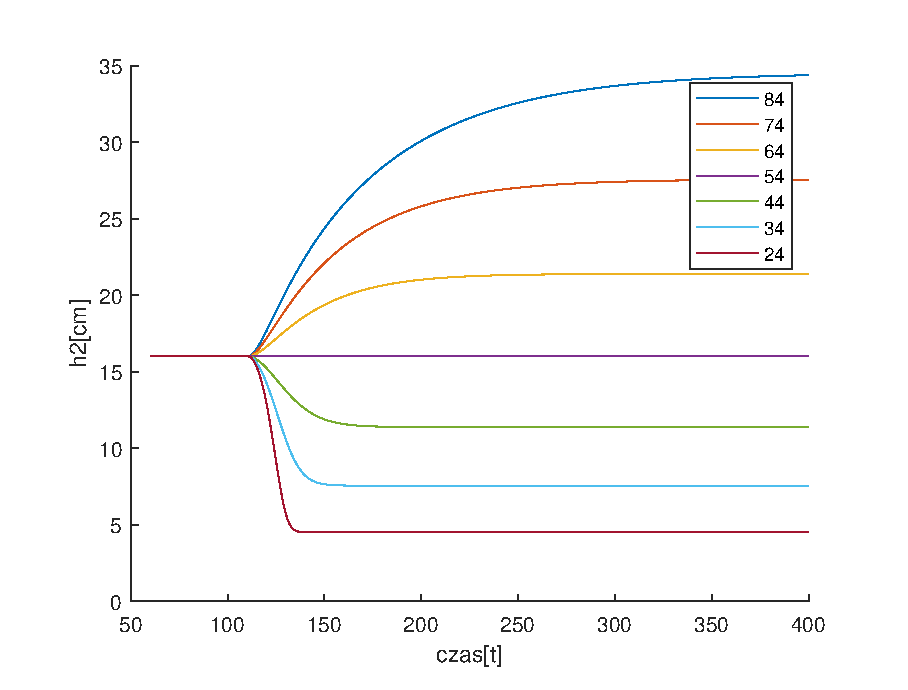
\includegraphics[width=0.9\linewidth]{plots/z1_model_u.eps}
			\caption{Przebiegi wyjścia dla skoku wartości sterowania w chwili 60s}
			\label{rys:model_u}
		\end{figure}
		\begin{figure}
			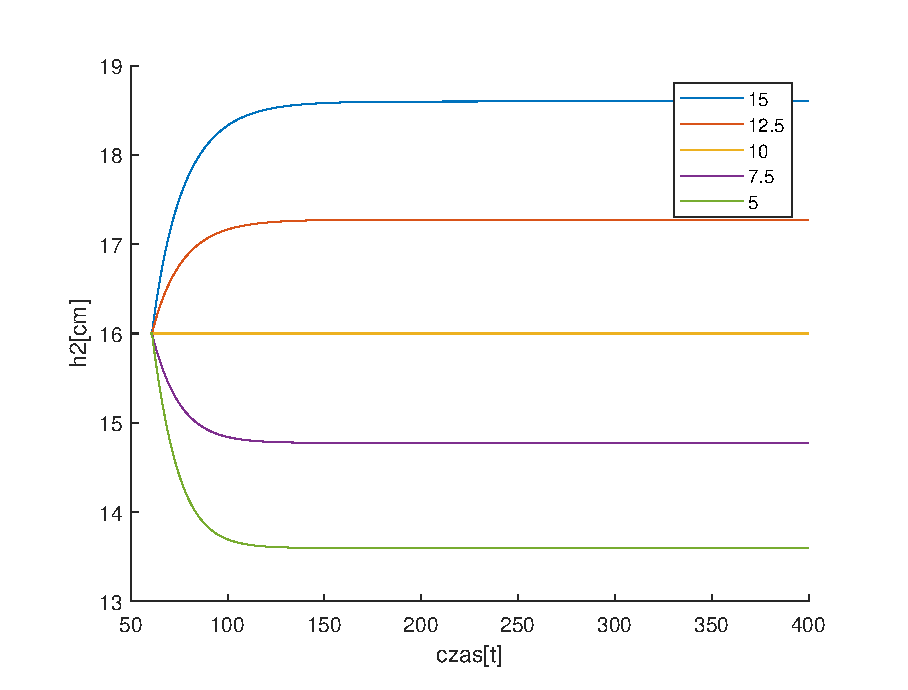
\includegraphics[width=0.9\linewidth]{plots/z1_model_z.eps}
			\caption{Przebiegi wyjścia dla skoku wartości sterowania w chwili 60s}
			\label{rys:model_z}
		\end{figure}
		\newpage

	\section{Model liniowy}
		\label{sec:model_lin}
		W celu uzyskania modelu liniowego należy zlinearyzować równania obiektu w podanym punkcie pracy. Zlinearyzowane równania wyglądają następująco:
		\begin{equation}
			\left\{
			\begin{tabular}{l}
				$V_1(k) =V_1(k-1) + (F_1(k-1)-F_{10}) + (F_D(k-1)-F_{D0}) -\frac{\alpha_1}{2\sqrt{h_{10}}}*(h_1(k-1)-h_{10}) $ \\\\
				$V_2(k) = V_2(k-1)+\frac{\alpha_1}{2\sqrt{h_{10}}}*(h_1(k-1)-h_{10}) - \frac{\alpha_2}{2\sqrt{h_{20}}}*(h_2(k-1)-h_{20})$\\\\
				$h_1(k) = h_{10}+\frac{1}{2\sqrt{C_1*V_{10}}}*(V_1(k)-V_{10})$\\\\
				$h_2(k) = h_{20}+\frac{1}{2\sqrt{C_2*V_{20}}}*(V_2(k)-V_{20})$\\\\
				$F_1(k) = F_{1in}(k-50)$
			\end{tabular}
			\right.
			\label{eq:lin}
		\end{equation}
		
		O ile $F_{10}$, $F_{D0}$ oraz $h_{10}$ mamy podane, tak $V_{10}$, $V_{20}$ oraz $h_{10}$ musimy sobie określić. Nie jest to złożone zadanie. W punkcie pracy pochodne obydwu objętości musi być zerowa, z czego wynika, że $F_2 = F_3 => \alpha_1*\sqrt{h_1} = \alpha_2*\sqrt{h_2}$. Ponieważ $\alpha_1 = \alpha_2$ to wysokość wody w punkcie pracy musi być taka sama dla obydwu zbiorników. Mając wysokości wody w obu zbiornikach można obliczyć jej objętość.
		
		Dla uzyskanego w ten sposób modelu liniowego przeprowadzono takie same testy jak dla oryginalnego modelu. Wynik testów przedstawiony jest na wykresach \ref{rys:modellin_u} oraz \ref{rys:modellin_z}, na których niebieskim kolorem widnieją przebiegi oryginalne, a różowym te dla obiektu zlinearyzowanego. Dla skoków sterowania do 44 oraz 64 przebiegi dla obydwu modeli są dosyć podobne zarówno kształtem jak i wartościami. Dla wysokich oraz niskich wartości nie jest już niestety tak dobrze. Obiekt liniowy ,w przeciwieństwie do oryginału, działa z taką samą dynamiką dla całego zakresu, co oznacza, że dla wysokich wartości sterowania jest on od niego szybszy, a dla niskich wolniejszy. Co więcej im dalej od punktu pracy tym większa różnica w wartości końcowej wyjścia. Dla skoków zakłócenia osiągane wartości są zbliżone dla skoków do 7.5 i 12.5. Niższe oraz wyższe spadki powodują coraz większe odchylenie końcowej wartości wyjścia, choć i tak wciąż nie jest ono bardzo duże. Jeśli chodzi o dynamikę obiekt zlinearyzowany reaguje na zmianę zakłócenia nieco wolniej niż obiekt oryginalny.
		
		\begin{figure}
			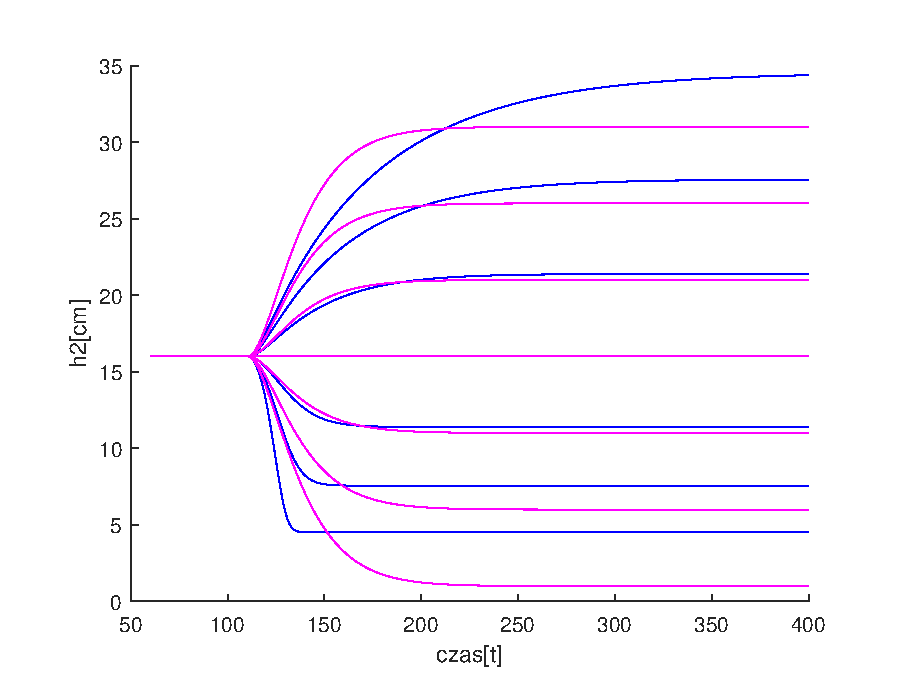
\includegraphics[width=0.9\linewidth]{plots/z1_modellin_u.eps}
			\caption{Przebiegi wyjścia dla skoku wartości sterowania w chwili 60s, dla modelu nieliniowego i liniowego}
			\label{rys:modellin_u}
		\end{figure}
		\begin{figure}
			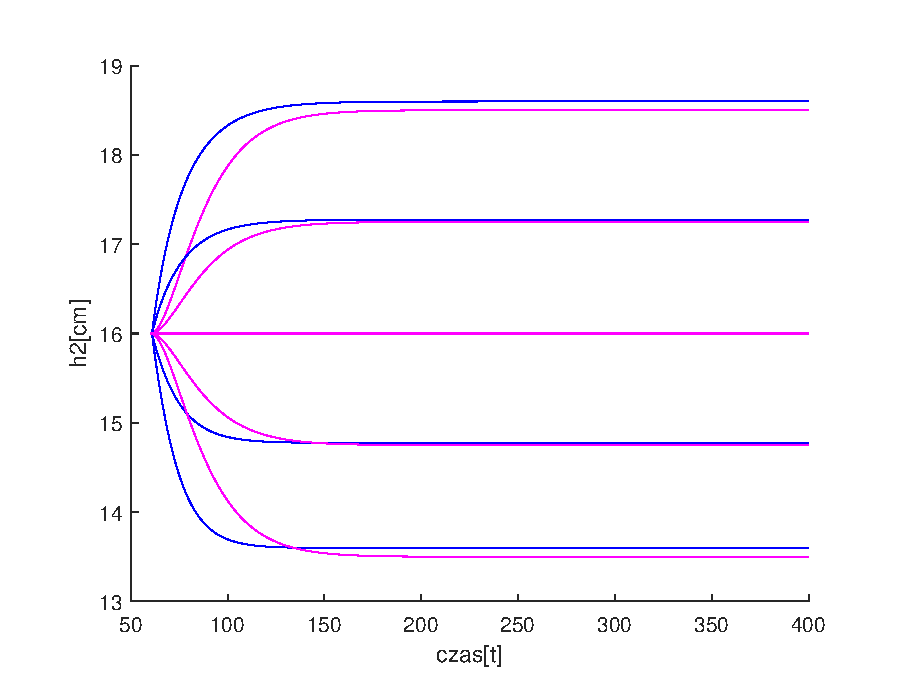
\includegraphics[width=0.9\linewidth]{plots/z1_modellin_z.eps}
			\caption{Przebiegi wyjścia dla skoku wartości sterowania w chwili 60s, dla modelu nieliniowego i liniowego}
			\label{rys:modellin_z}
		\end{figure}
		\newpage
	
	\section{Regulator}
		\label{sec:dmc}
		Tworząc regulator dla posiadanego obiektu zdecydowaliśmy się na regulator predykcyjny DMC. Nasza decyzja wynikała z faktu możliwości uzyskania przez nas niezaszumionej odpowiedzi skokowej obiektu na skok sterowania oraz skok zakłócenia oraz z faktu, że stosowanie regulatora DMC w formie GPC jesteśmy w stanie uwzględnić zakłócenie w regulatorze.
		
		W celu uzyskania odpowiedzi skokowych wykorzystaliśmy obiekt zlinearyzowany w punkcie pracy. Wykonując skok sterowania z punktu pracy otrzymaliśmy przebieg wyjścia obiektu. Następnie odjeliśmy od przebiegu wartość wyjścia w punkcie pracy i podzieliliśmy przez długość skoku sterowania, zgodnie z wzorem \ref{eq:skokowa}, otrzymując w ten sposób znormalizowaną odpowiedź skokową. Dla odpowiedzi skokowej zakłócenia postąpiliśmy analogicznie wykonując skok zakłócenia i dzieląc na końcu przez długość tegoż skoku. Wygląd obydwu odpowiedzi przedstawiony został na wykresie \ref{rys:skok}.
		
		\begin{equation}
			s = \frac{y-y_0}{\Delta u}
			\label{eq:skokowa}
		\end{equation}
		
		\begin{figure}[h!]
			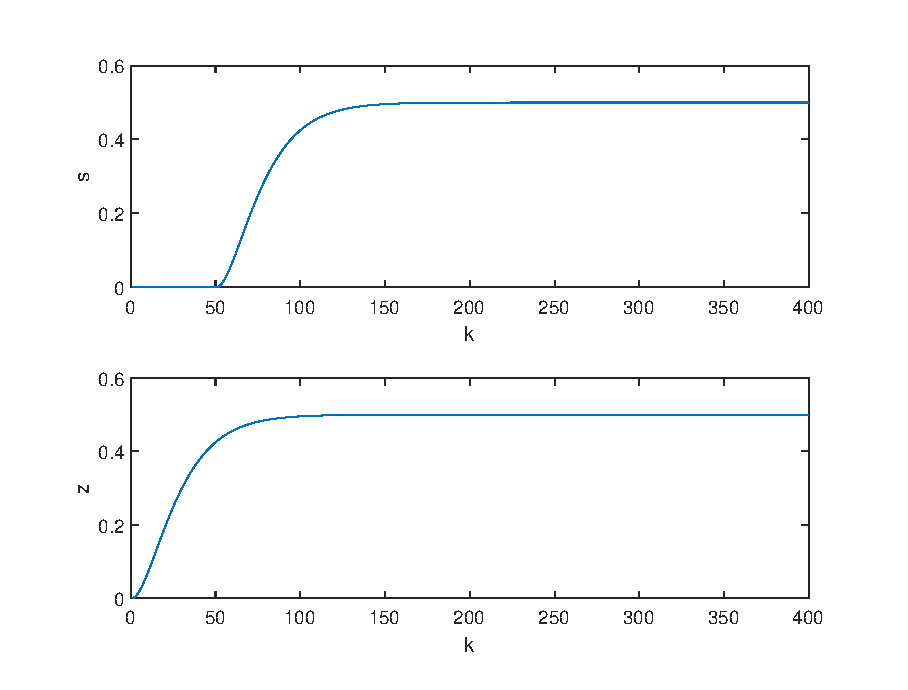
\includegraphics[width=0.9\linewidth]{plots/z1_step.eps}
			\caption{Odpowiedzi skokowe dla skoku sterowania(s) i zakłócenia(z)}
			\label{rys:skok}
		\end{figure}
	
		Do obliczania regulacji DMC używaliśmy regulatora w formie analitycznej, określonego wzorami od \ref{yzadm} do \ref{dU1}:
		
		\begin{equation}
		\boldsymbol{Y}^{\mathrm{zad}}(k)=\left[
		\begin{array}{c}
		Y^{\mathrm{zad}}(k)\\
		\vdots\\
		Y^{\mathrm{zad}}(k)
		\end{array}
		\right]_{\mathrm{Nx1}}
		\label{yzadm}
		\end{equation}
		
		\begin{equation}
		\boldsymbol{Y}(k)=\left[
		\begin{array}{c}
		y(k)\\
		\vdots\\
		y(k)
		\end{array}
		\right]_{\mathrm{Nx1}}
		\label{ym}
		\end{equation}
		
		\begin{equation}
		\triangle\boldsymbol{U}(k)=\left[
		\begin{array}{c}
		\triangle u(k|k)\\
		\vdots\\
		\triangle u(k+N_u -1 |k)
		\end{array}
		\right]_{\mathrm{N_ux1}}
		\label{dUm}
		\end{equation}
		
		\begin{equation}
		\triangle\boldsymbol{U^P}(k)=\left[
		\begin{array}{c}
		\triangle u(k-1)\\
		\vdots\\
		\triangle u(k-(D-1))
		\end{array}
		\right]_{\mathrm{(D-1)x1}}
		\label{dUPm}
		\end{equation}
		
		\begin{equation}
		\boldsymbol{M}=\left[
		\begin{array}
		{cccc}
		s_{1} & 0 & \ldots & 0\\
		s_{2} & s_{1} & \ldots & 0\\
		\vdots & \vdots & \ddots & \vdots\\
		s_{N} & s_{N-1} & \ldots &  s_{N-N_{\mathrm{u}}+1}
		\end{array}
		\right]_{\mathrm{NxN_u}}
		\label{Mm}
		\end{equation}
		
		\begin{equation}
		\boldsymbol{M^P}=\left[
		\begin{array}
		{cccc}
		s_{2}-s_{1} & s_{3}-s_{2} & \ldots & s_{D}-s_{D-1}\\
		s_{3}-s_{1} & s_{4}-s_{2} & \ldots & s_{D+1}-s_{D-1}\\
		\vdots & \vdots & \ddots & \vdots\\
		s_{N+1}-s_{1} & s_{N+2}-s_{2} & \ldots &  s_{N+D-1}-S_{D-1}
		\end{array}
		\right]_{\mathrm{NxD-1}}
		\label{MPm}
		\end{equation}
		
		\begin{equation}
		\boldsymbol{M^{zP}}=\left[
		\begin{array}
		{ccccc}
		sz_{1} & sz_{2}-sz_{1} & sz_{3}-sz_{2} & \ldots & sz_{D_z}-sz_{D_z-1}\\
		sz_{2} & sz_{3}-sz_{1} & sz_{4}-sz_{2} & \ldots & sz_{D_z+1}-sz_{D_z-1}\\
		\vdots & \vdots & \vdots & \ddots & \vdots\\
		sz_{N} & sz_{N+1}-sz_{1} & sz_{N+2}-sz_{2} & \ldots &  sz_{N+D_z-1}-sz_{D_z-1}
		\end{array}
		\right]_{\mathrm{NxDz}}
		\label{MPzm}
		\end{equation}
		
		\begin{equation}
		Y^0(k)=Y(k)+M^P\triangle U^P(k)+M^{zP}\triangle  Z^P(k)
		\label{Y0z}
		\end{equation}
		
		\begin{equation}
		K=(M^TM+\lambda*I)^{-1}M^T
		\label{K}
		\end{equation}
		
		\begin{equation}
		\triangle U(k)=K(Y^{zad}(k)-Y^0(k))
		\label{dU1}
		\end{equation}
		
		W naszej regulacji potrzebujemy wyznaczyć tylko pierwszy element macierzy $\triangle U(k)$ czyli $\triangle u(k|k)$. W tym celu rozwijamy wzór do postaci:
		
		\begin{equation}
		\triangle u(k|k)=k_ee(k)-k_u\triangle\boldsymbol U^P-k_z\triangle\boldsymbol Z^P
		\label{dukkz}
		\end{equation}
		
		gdzie:
		
		\begin{equation}
		e(k)=Y^{zad}(k)-Y(k)
		\label{e}
		\end{equation}
		
		\begin{equation}
		k_e=\sum_{i=1}^N K(1,i)
		\label{ke}
		\end{equation}
		
		\begin{equation}
		k_u=kM^P
		\label{ku}
		\end{equation}
		
		\begin{equation}
		k_z=kM^{zP}
		\label{kz}
		\end{equation}
		
		k to oznaczenie pierwszego wiersza macierzy K. Aktualne sterowanie otrzymujemy poprzez zsumowanie poprzedniego sterowania i aktualnie wyliczonego $\triangle u(k|k)$. 
		
		Po implementacji przystąpiliśmy do testowania regulatora. W tym celu zadaliśmy mu przebieg zakładający 4 zmiany wartości zadanej oraz 4 zmiany zakłócenia. Testowanie obiektu wymagało od nas także dobrania horyzontów oraz wartości lambda. Co do horyzontów, ponieważ zmniejszanie ich nie może poprawić regulacji pozostaliśmy przy stałej wartości równej odpowiedzi skokowej. Jeśli chodzi o lambda dla bardzo małych wartości przebiegi były nieakceptowalne. Poniżej przedstawiliśmy przebiegi regulacji dla trzech różnych lambd: 100, 2000 oraz 10000. Dla tych trzech przebiegów obliczony został średni błąd kwadratowy regulacji określony wzorem \ref{eq:blad}. Dla poszczególnych przebiegów błąd ten wynosił:
		\begin{itemize}
			\item lambda 100 - 13.2852
			\item lambda 2000 - 18.4502
			\item lambda 10000 - 27.1046
		\end{itemize}
		Dla lambdy 100 błąd jest definitywnie najmniejszy, jednakże zarówno sterowanie jak i wyjście ulegają znacznym oscylacjom. Sytuacja dla lambda 10000 jest odwrotna, oscylacji brak, jednakże błąd wzrósł dwukrotnie. Lambda 2000 jest najlepszym rozwiązaniem z przetestowanych, oscylacje są obecne, jednakże błąd nie jest aż taki wysoki
		
		\begin{equation}
			e = \frac{\sum_{t=1}^{t_{max}}(y_{zad}(t)-y(t))^2}{t_{max}}
			\label{eq:blad}
		\end{equation}
		
		
		\begin{figure}
			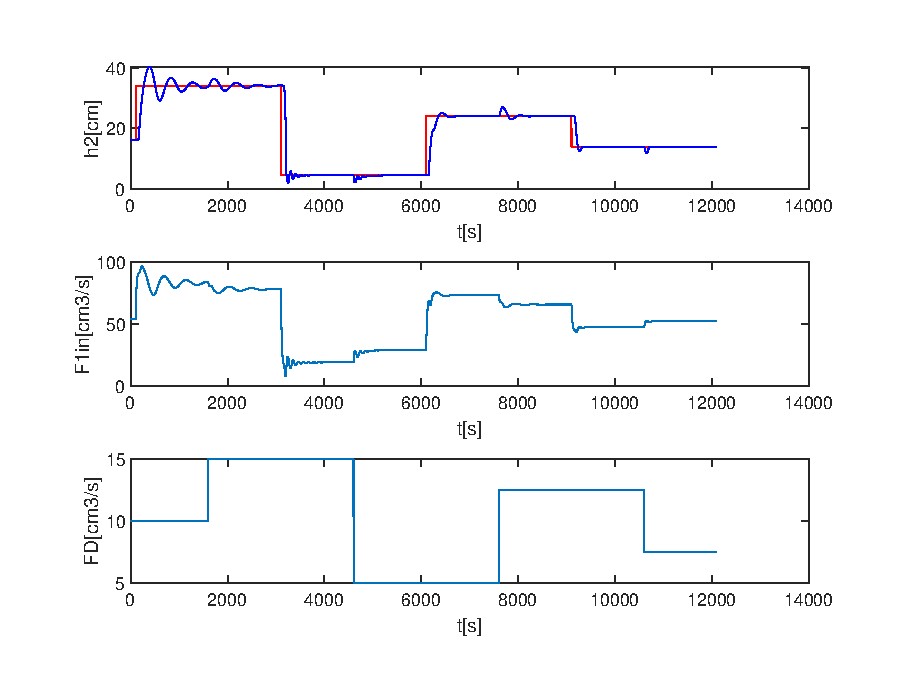
\includegraphics[width=0.9\linewidth]{plots/z1_dmc_100.eps}
			\caption{Przebieg regulacji dla lambda = 100}
			\label{rys:dmc100}
		\end{figure}
		
		\begin{figure}
			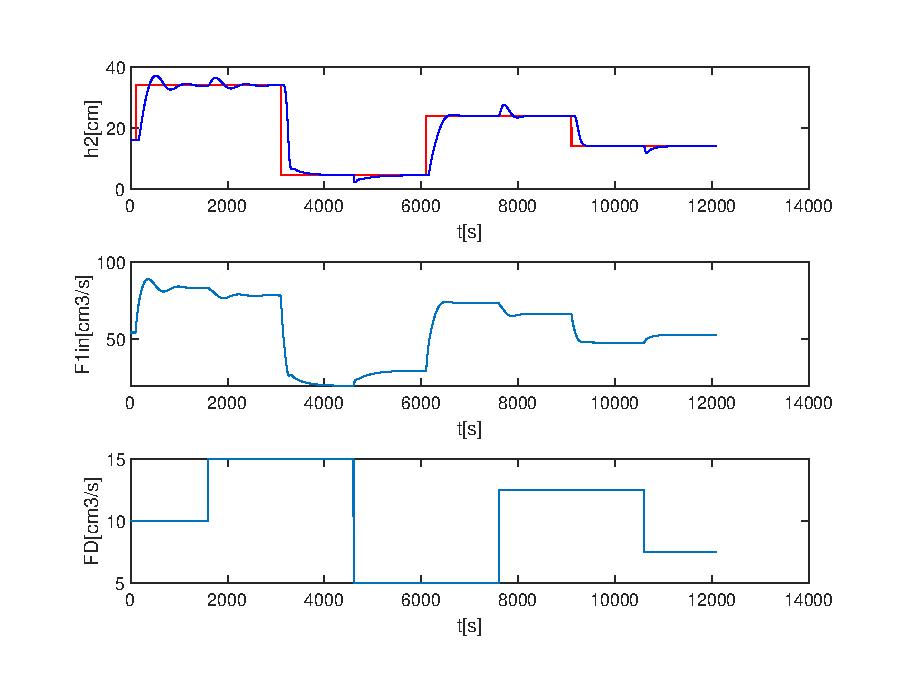
\includegraphics[width=0.9\linewidth]{plots/z1_dmc_2000.eps}
			\caption{Przebieg regulacji dla lambda = 2000}
			\label{rys:dmc1000}
		\end{figure}
		
		\begin{figure}
			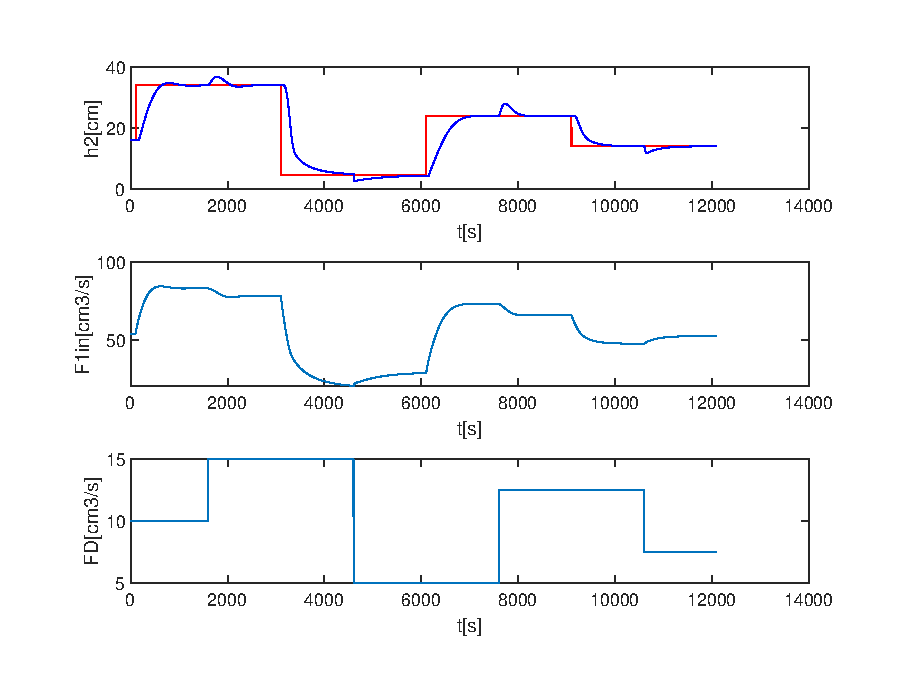
\includegraphics[width=0.9\linewidth]{plots/z1_dmc_10000.eps}
			\caption{Przebieg regulacji dla lambda = 10000}
			\label{rys:dmc10000}
		\end{figure}
	\newpage
	\chapter{Zadanie 2}
	\label{ch:zadanie2}
	
	\section{Obiekt rozmyty}
		\label{sec:ob_roz}
		Utworzenie modelu rozmytego Takagi-Sugeno dla obiektu należy zacząć od wyznaczenia funkcji przynależności. Jako funkcji przynależności zdecydowaliśmy się użyć funkcji sigmoidalnych. Ponieważ projekt zakłada utworzenie modeli rozmytych z dwoma, trzema, czterema oraz pięcioma modelami lokalnymi, funkcje przynależności dla pierwszego, n-tego oraz ostatniego (przy r obecnych modelach lokalnych) modelu lokalnego wyglądają tak jak w równaniach od \ref{eq:sig1} do \ref{eq:sigost}. W podanych wzorach zmienna a oznacza nachylenie funkcji i została przyjęta taka sama dla wszystkich modeli lokalnych. Wektor c natomiast zawiera punkty dla których funkcje przynależności sąsiednich modeli lokalnych osiągają wartość 0.5. Wartość a została dobrana eksperymentalnie na poziomie a=3. Wartości c zostały wyliczone poprzez podzielenie zakresu wartości zmiennej na podstawie której liczony jest obiekt rozmyty przez ilość regulatorów lokalnych, co zagwarantowało w równomierny podział zbiorów rozmytych. Zdecydowaliśmy się na wykorzystanie wyjścia obiektu jako zmiennej determinującej zbiory rozmyte. Decyzja ta poparta była faktem, że dla sterowania w obiekcie występuje znaczne opóźnienie co prawdopodobnie uniemożliwiłoby późniejsze zaimplementowanie na utworzonych zbiorach rozmytych skutecznie działającego regulatora. Dla badanego w zadaniu pierwszym zakresu sterowań wyjście obiektu przyjmuje wartości w przybliżeniu od 4.5 do 34.5, dlatego właśnie w takim zakresie tworzone były zbiory rozmyte. Dodatkowo dla każdego zbioru rozmytego należało określić punkt pracy w którym zlinearyzowany był obiekt lokalny. Punkty pracy zostały wyznaczone na podstawie kształtu poszczególnych funkcji przynależności. Wartość wyjścia w punkcie pracy dla wybranego modelu równa jest w przybliżeniu wartości wyjścia znajdującej się w środku przedziału dla którego funkcja przynależności wynosi 1. Funkcje przynależności dla utworzonych obiektów rozmytych przedstawione zostały na wykresach od \ref{rys:roz2} do \ref{rys:roz5}.
		
		\begin{equation}
			\mu(1) = 1-\frac{1}{1+e^{-a*(h2-c(1))}}
			\label{eq:sig1}
		\end{equation}
		\begin{equation}
			\mu(n) = \frac{1}{1+e^{-a*(h2-c(n-1))}}-\frac{1}{1+e^{-a*(h2-c(n))}}
			\label{eq:sign}
		\end{equation}
		\begin{equation}
		\mu(r) = \frac{1}{1+e^{-a*(h2-c(r-1))}}
		\label{eq:sigost}
		\end{equation}
		
		\begin{figure}[h!]
			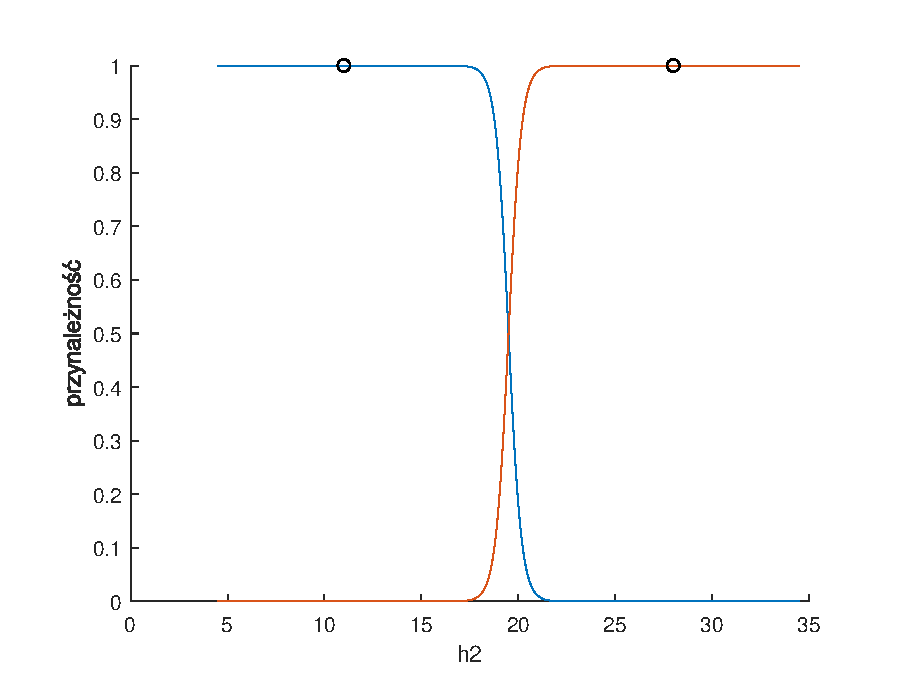
\includegraphics[width=0.9\linewidth]{plots/z2_modelroz_2.eps}
			\caption{Funkcje przynależności dla obiektu rozmytego z dwoma obiektami lokalnymi}
			\label{rys:roz2}
		\end{figure}
		\begin{figure}[h!]
			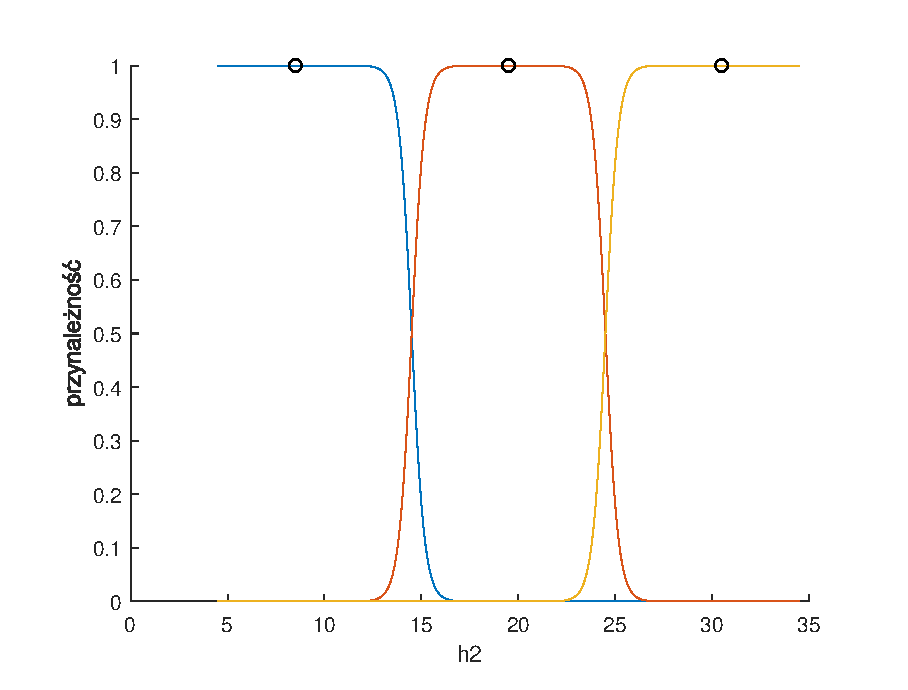
\includegraphics[width=0.9\linewidth]{plots/z2_modelroz_3.eps}
			\caption{Funkcje przynależności dla obiektu rozmytego z trzema obiektami lokalnymi}
			\label{rys:roz3}
		\end{figure}
		\begin{figure}[h!]
			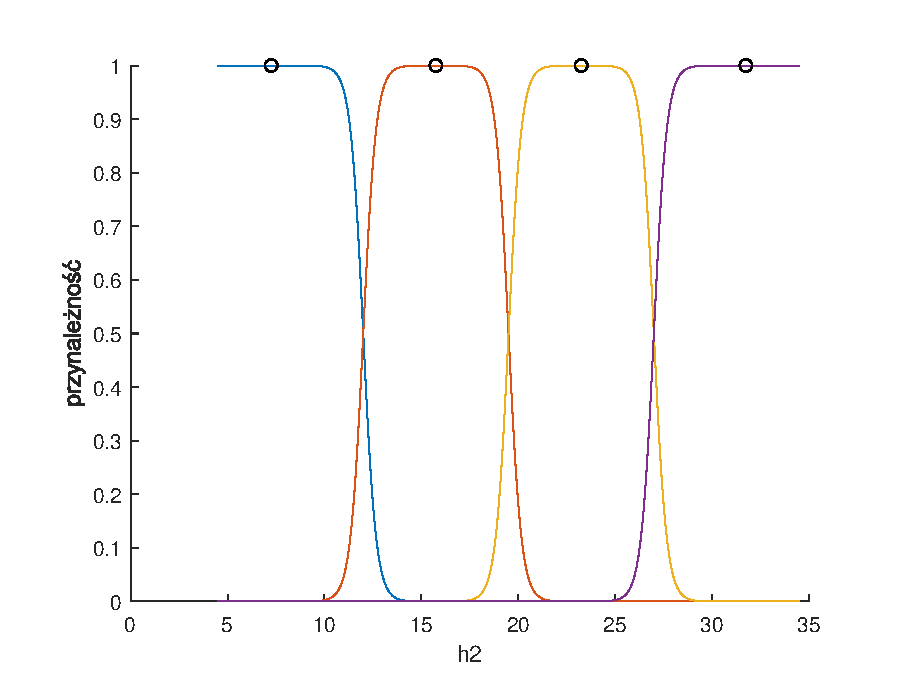
\includegraphics[width=0.9\linewidth]{plots/z2_modelroz_4.eps}
			\caption{Funkcje przynależności dla obiektu rozmytego z czterema obiektami lokalnymi}
			\label{rys:roz4}
		\end{figure}
		\begin{figure}[h!]
			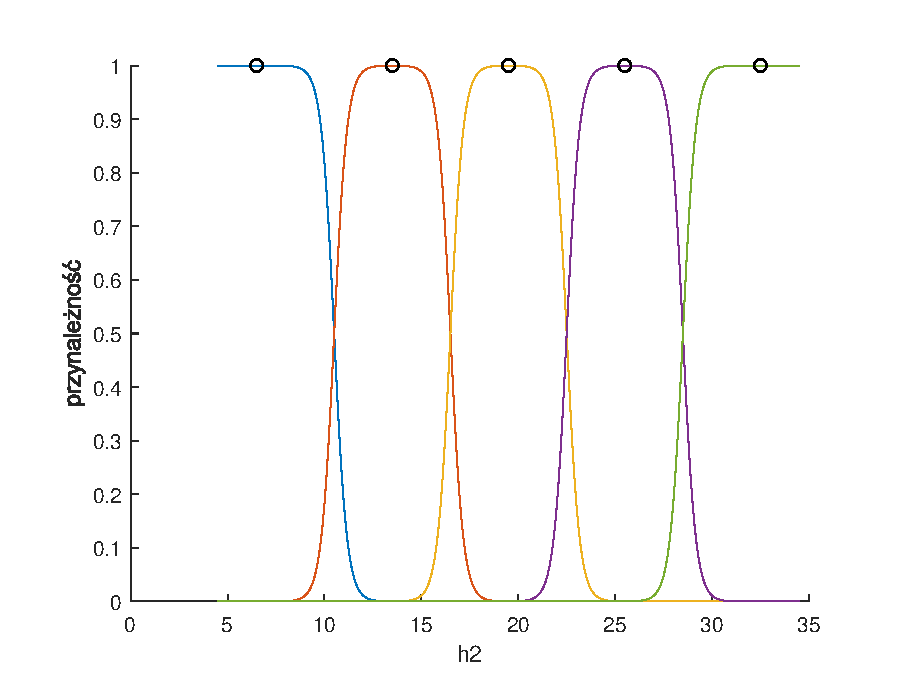
\includegraphics[width=0.9\linewidth]{plots/z2_modelroz_5.eps}
			\caption{Funkcje przynależności dla obiektu rozmytego z pięcioma obiektami lokalnymi}
			\label{rys:roz5}
		\end{figure}
	
	
		Utworzenie obiektu rozmytego na podstawie przedstawionych funkcji przynależności nie sprawiło już zbytniego problemu. Zakładając, że obiekt ma określoną ilość zbiorów rozmytych i każdy zbiór posiada swój punkt linearyzacji zaimplementowane została określona ilość obiektów liniowych. W każdej iteracji liczone są wyjścia wszystkich obiektów liniowych oraz wagi według funkcji przynależności. Następnie faktyczny stan obiektu otrzymywany jest poprzez przemnożenie wyników lokalnych przez ich wagi i podzielenie otrzymanej liczby przez sumę wag. Oczywiście dla każdego modelu liniowego potrzebny jest punkt linearyzacji, który jak już wspominałem został określony jedynie poprzez wartość wyjścia obiektu $h_{20}$. Wartości $V_{10}$, $V_{20}$ oraz $h_{10}$ obliczane są analogicznie jak dla obiektu liniowego z pierwszego zadania. Co do wartości zakłócenia $F_{D0}$ ustalona została ona na 10. Wartość sterowania w punkcie linearyzacji $F_{10}$ można zatem wyliczyć podstawiając wartość 0 pod pochodną $dV/dt$, co daje nam działanie $F_{10} = \alpha_1*\sqrt{h_{20}}-F_{D0}$.
		
		Porównania działania poszczególnych modeli rozmytych modelem nieliniowym oraz liniowym obiektu przedstawione zostały na wykresach od \ref{rys:roz2p} do \ref{rys:roz5p}. Dla każdego modelu wykonane zostały przebiegi ze skokami sterowania w kroku 100. Użyte skoki sterowania są takie same jak w zadaniu pierwszym. Na wykresach przebiegi dla oryginalnego obiektu przedstawione są kolorem niebieskim, dla zlinearyzowanego różowym, a dla rozmytego zielonym.
		
		Dla modelu z dwoma obiektami lokalnymi działanie modelu rozmytego definitywnie nie jest zadowalające. Końcowa wartość wyjścia obiektu rozmytego w większości przypadków zauważalnie rozbiega się z końcową wartością dla oryginalnego modelu. Kształty przebiegów dla poszczególnych skoków nie są podobne do przebiegów nieliniowego ani liniowego obiektu. Przebiegiem, który najbardziej pokrywa się z oryginałem jest ten dla skoku sterowania do 34 (drugi od dołu).
		
		Dla modelu z trzema obiektami lokalnymi sytuacja wydaje się lepsza. Przebiegi dla skoków powyżej punktu pracy są zbliżone w wyglądzie do oryginalnego obiektu. Nie licząc przebiegu dla skoku sterowania do 24 (pierwszy od dołu) wartości końcowe wyjścia obiektu rozmytego w przybliżeniu pokrywają się z wartościami dla obiektu oryginalnego.
		
		Dla modelu z czterema obiektami lokalnymi znowu nastąpiła nieznaczna poprawa. Przebiegi przez większość symulacji pokrywają się kształtem z przebiegami dla pierwotnego modelu, jednakże część wartości końcowych wyjścia nieznacznie odbiega od pożądanych.

		Modelu z pięcioma obiektami lokalnymi działa najlepiej z przedstawionych. Poza kilkoma miejscami przebiegi pokrywają się z przebiegami dla oryginalnego obiektu. Wartości końcowe także są w przybliżeniu równe wartościom końcowym dla obiektu oryginalnego. Obiekt ten jest zdecydowanie najlepszym z utworzonych i to właśnie on wykorzystywany będzie do dalszych badań.
		
		Badanie to ukazuje jak przydatne mogą być modele rozmyte przy modelowaniu obiektów nieliniowych. Działanie modelu liniowego w dużej odległości od punktu pracy zbyt znacząco różniło się od działania modelu nieliniowego, by można było stosować je zamiennie. Dzięki wykorzystaniu kilku modeli liniowych sprzężonych w model rozmyty jesteśmy w stanie dosyć dokładnie odwzorować obiekt, co potencjalnie umożliwiałoby stosowanie modelu rozmytego zamiast oryginału.
		
		Pomimo prób nie udało się znaleźć lepszego modelu rozmytego, czyli takiego, który niwelowałby znacząco wady modelu otrzymanego automatycznie (różnice w przebiegach funkcji dla skoków do niskich sterowań) nie pogarszając działania reszty modelu. Z tego powodu podtrzymaliśmy naszą decyzję o używaniu wygenerowanych dla 5 modeli lokalnych funkcji przynależności.
		
		\begin{figure}[h!]
			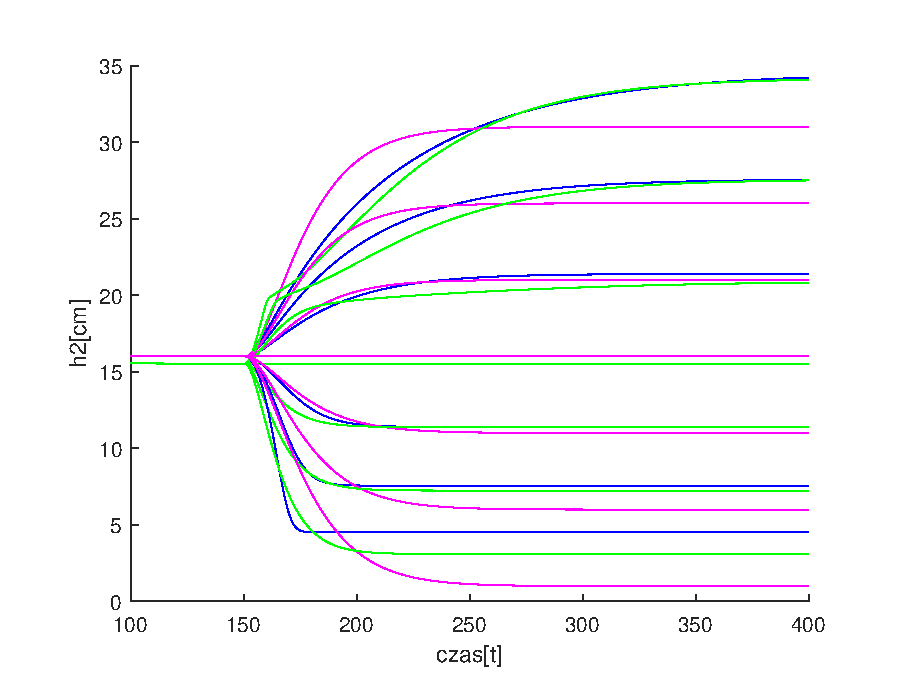
\includegraphics[width=0.9\linewidth]{plots/z2_modelroz_2p.eps}
			\caption{Porównanie działania dla obiektu rozmytego z dwoma obiektami lokalnymi}
			\label{rys:roz2p}
		\end{figure}
		\begin{figure}[h!]
			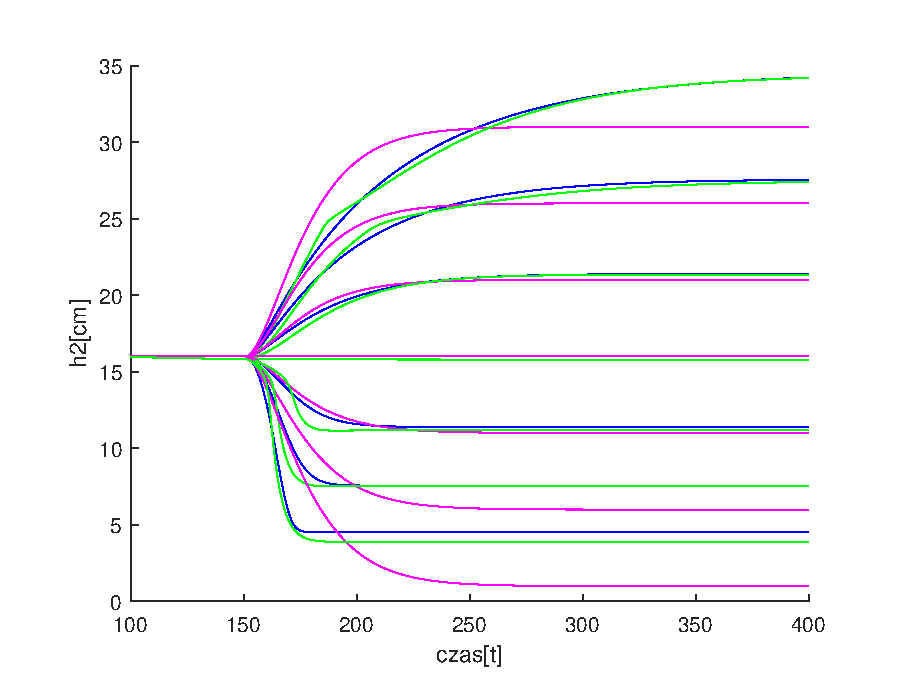
\includegraphics[width=0.9\linewidth]{plots/z2_modelroz_3p.eps}
			\caption{Porównanie działania dla obiektu rozmytego z trzema obiektami lokalnymi}
			\label{rys:roz3p}
		\end{figure}
		\begin{figure}[h!]
			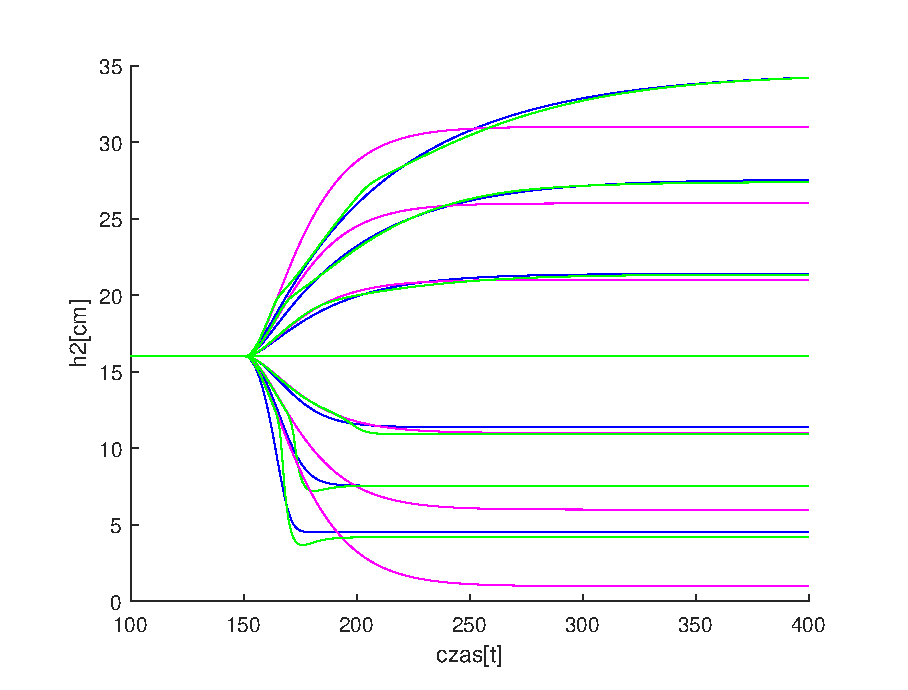
\includegraphics[width=0.9\linewidth]{plots/z2_modelroz_4p.eps}
			\caption{Porównanie działania dla obiektu rozmytego z czterema obiektami lokalnymi}
			\label{rys:roz4p}
		\end{figure}
		\begin{figure}[h!]
			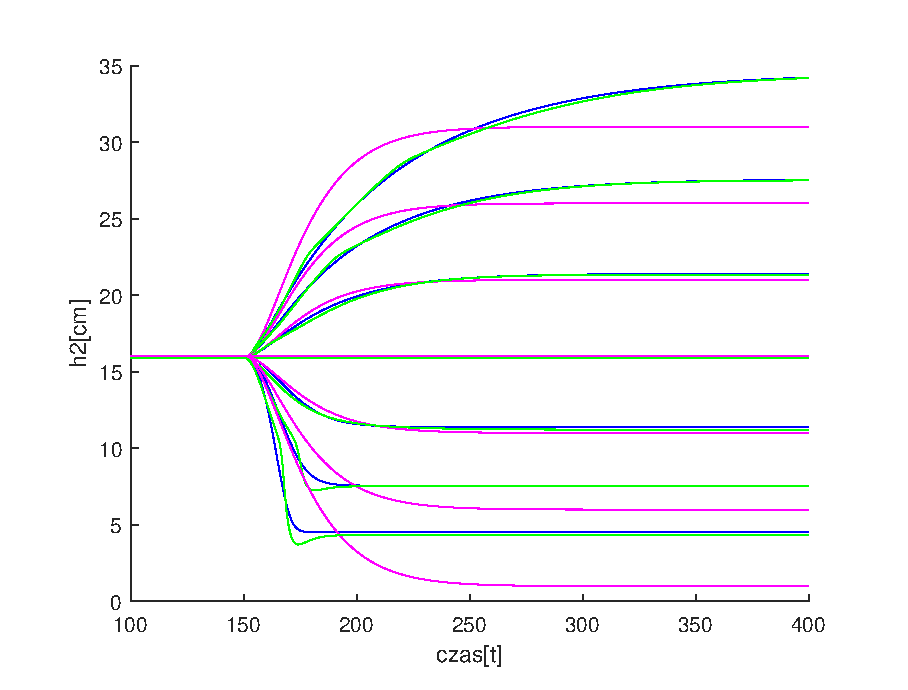
\includegraphics[width=0.9\linewidth]{plots/z2_modelroz_5p.eps}
			\caption{Porównanie działania dla obiektu rozmytego z pięcioma obiektami lokalnymi}
			\label{rys:roz5p}
		\end{figure}
	\newpage
	\section{DMC rozmyty}\
		Implementacja rozmytego regulatora DMC nie jest bardzo skomplikowana. W tym celu należy zaimplementować tyle regulatorów DMC ile jest zbiorów rozmytych, w naszym wypadku 5. Regulatory różnią się między sobą odpowiedziami skokowymi, które są zebrane w punktach pracy odpowiadających każdemu z modelów. W każdym kroku regulacji każdy z regulatorów lokalnych oblicza zmianę sterowania. Następnie obliczane są wagi poszczególnych zbiorów rozmytych i następuje rozmycie zmiany sterowania. Każde z wyliczonych sterowań przemnażane jest przez swoją wagę, wyniki sumuje się i dzieli przez sumę wag otrzymując w ten sposób końcową zmianę sterowania.
		
		Dodatkowo w wymaganiach napisane było, że regulator rozmyty powinien posiadać ograniczenia. W tym celu przyjęte zostały przez nas: maksymalna wartość sterowania - 90, minimalna wartość sterowania - 20 oraz maksymalna zmiana sterowania w jednym kroku - 1. Ograniczenia te uwzględnia się dopiero po obliczeniu końcowej wartości zmiany sterowania.
		
		Stworzony na podstawie wyznaczonych funkcji przynależności regulator rozmyty otrzymał takie same zadanie wyregulowania obiektu jak zwykły regulator w zadaniu pierwszym. Początkowo wartości wszystkich horyzontów zostały ustawione na najwyższą wartość, czyli długość odpowiedzi skokowej - 400, a lambda na wartość dla której przebieg zwykłego regulatora wydał nam się optymalny - 2000. Przebiegi regulacji obiektu dla tych parametrów zostały przedstawione na wykresie \ref{rys:dmcoryg}. Jak widać przebiegi są bardzo dobre, a w porównaniu z przebiegami pojedynczego DMC dla tej samej lambdy wręcz genialne. Błąd regulacji także jest mniejszy i wynosi 18.2898. Obiekt dąży do zadanej wartości wyjścia bez oscylacji ani przesterowań i osiąga go dość szybko.
		
		Po tak spektakularnym sukcesie oryginalnego kształtu funkcji rozpoczęliśmy eksperymenty nad jego zmianą w celu dalszej optymalizacji regulacji. Po wielu próbach przystaliśmy na kształt przedstawiony na rysunku \ref{rys:dmcprzyn}. Przebieg regulacji dla tak skonstruowanych zbiorów rozmytych przedstawiony jest na wykresie \ref{rys:dmcroz2000}. Jak widać nie uległ on znaczącej zmianie. Błąd regulacji dla zmienionej funkcji przynależności wyniósł jednak nieco mniej, a dokładnie 18.2504.
		
		Po zmianie właściwości rozmycia zdecydowaliśmy się jeszcze sprawdzić działanie dla mniejszych wartości lambda, a dokładnie dla lambda równego 100, dla którego oryginalny DMC nie radził sobie dobrze z regulacją, powodując gasnące oscylacje dla wysokich skoków wartości zadanej. Przebieg dla zmniejszonej lambdy przedstawiony został na wykresie \ref{rys:dmcroz100}. Jak widać uległ on nieco pogorszeniu, zaczęły występować niewielkie przesterowania oraz pojedyncze oscylacje. Z drugiej strony błąd sterowania zmalał prawie o jedną trzecią swojej dotychczasowej wartości, aż do 13.6096. Zdecydowaliśmy, że niewielkie pogorszenie przebiegów jest małą ceną za znacznie niższy błąd i pozostaliśmy przy zmienionej wartości lambda.
		
		Ostatnią rzeczą jaką regulowaliśmy dla zaimplementowanego regulatora rozmytego jest zmiana długości horyzontów. Zdecydowaliśmy się na ten krok, choć zazwyczaj nie przynosi on poprawy regulacji, po części ze względu na kolejne zadania projektu, w których wymagane jest używanie algorytmów optymalizacji, znacznie spowalnianych przez dużą złożoność obliczeniową. Horyzonty skracane były przez nas do momentu, gdy błąd regulacji nie ulegał pogorszeniu. W ten sposób doszliśmy do następujących wartości horyzontów: D = 200, N = 150, Nu = 100, Dz = 200. Przebieg regulacji dla zmniejszonych horyzontów znajduje się na wykresie \ref{rys:dmcroz100hor}. Jak widać nie ma w nim widocznych zmian. Co ciekawe błąd regulacji dla skróconych horyzontów uległ nieznacznej poprawie, do poziomu 13.5395. Nie widząc żadnych przeciwwskazań zdecydowaliśmy o dalszym używaniu skróconych horyzontów w kolejnych zadaniach.
		
		W wykonanych w tym zadaniu przebiegach regulacji można zauważyć działanie ograniczenia wartości sterowania. Jeśli dokładnie przyjrzeć się wykresom zauważalne jest, że ustabilizowana wartość wyjścia obiektu dla czasu w okolicy 4000s jest nieznacznie większa od zadanej. Dzieje się tak, ponieważ sterowanie osiąga swoją wartość minimalną, co spowodowane jest równoczesną obecnością dużego zakłócenia. Przy wystąpieniu spadku zakłócenia w chwili 4600, regulatorowi po chwili udaje się bez problemu osiągnąć zadaną wartość. Ponieważ zachowanie to umożliwia zaobserwowanie zaimplementowanego ograniczenia nie zostało ono usunięte w kolejnych zadaniach, co mogłoby być wykonane dzięki nieznacznemu zwiększeniu dolnej granicy sterowania.
		
		\begin{figure}[h!]
			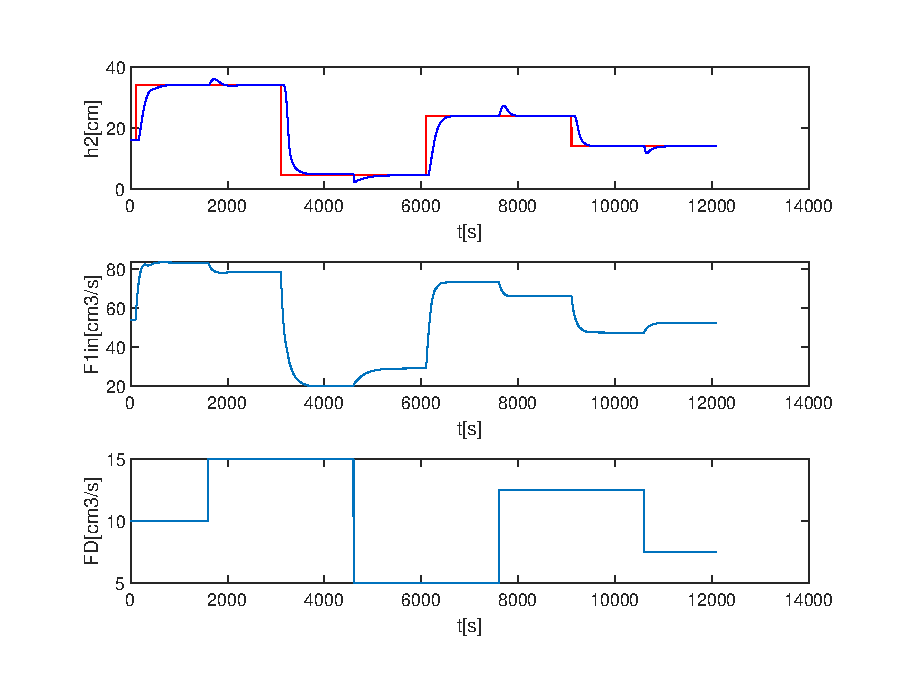
\includegraphics[width=0.9\linewidth]{plots/z2_dmc2000oryg.eps}
			\caption{Przebieg regulacji dla DMC rozmytego przy lambda 2000}
			\label{rys:dmcoryg}
		\end{figure}
		\begin{figure}[h!]
			\includegraphics[width=0.85\linewidth]{plots/z2_dmcprzyn.eps}
			\caption{Zmodyfikowane funkcje przynależności}
			\label{rys:dmcprzyn}
		\end{figure}
		\begin{figure}[h!]
			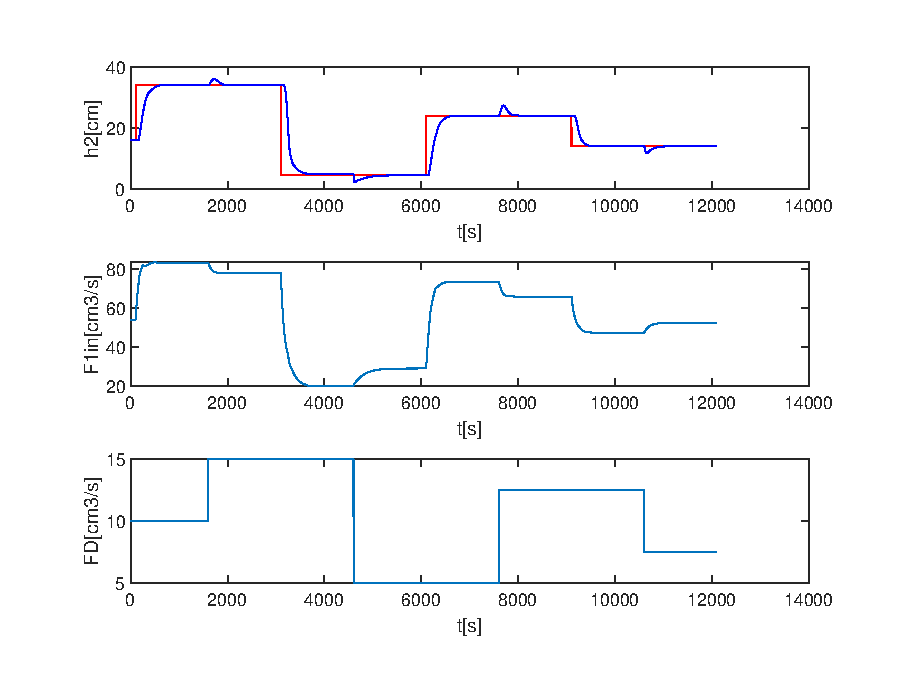
\includegraphics[width=0.9\linewidth]{plots/z2_dmc2000.eps}
			\caption{Przebieg regulacji dla DMC rozmytego przy lambda 2000 i zmodyfikowanych funkcjach przynależności}
			\label{rys:dmcroz2000}
		\end{figure}
		\begin{figure}[h!]
			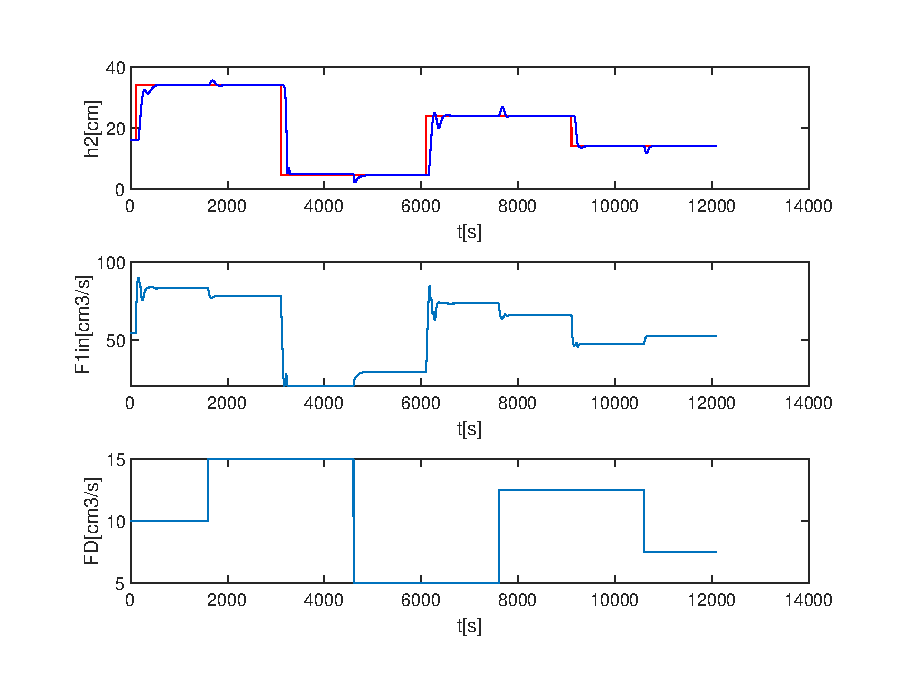
\includegraphics[width=0.9\linewidth]{plots/z2_dmc100.eps}
			\caption{Przebieg regulacji dla DMC rozmytego przy lambda 100}
			\label{rys:dmcroz100}
		\end{figure}
		\begin{figure}[h!]
			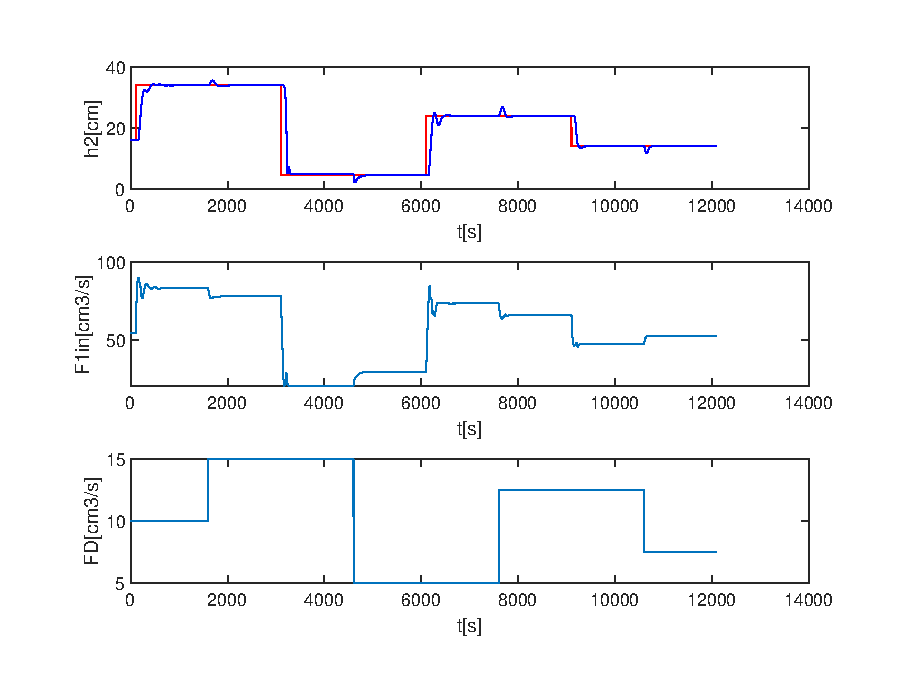
\includegraphics[width=0.9\linewidth]{plots/z2_dmchor.eps}
			\caption{Przebieg regulacji dla DMC rozmytego przy lambda 100 i skróconych horyzontach}
			\label{rys:dmcroz100hor}
		\end{figure}
		
	\chapter{Numeryczny rozmyty regulator SL}
	Rozmyty regulator typu SL jest w pewnym sensie podobny do rozmytego regulatora DMC, z dokładnością do tego, kiedy następuje rozmycie. Otóż w regulatorze SL rozmywana jest nie końcowa zmiana sterowania, a odpowiedzi skokowe regulatorów. W każdym kroku regulacji na podstawie poszczególnych odpowiedzi skokowych oraz aktualnych wag obliczana jest wspólna odpowiedź skokowa, a następnie następuje obliczane są nowe macierze $M$, $M^P$ i $M^{zP}$ na postawie których obliczana jest rozmyta odpowiedź swobodna obiektu, wykorzystywana do regulacji.
	
	Ponieważ wspomniany rozmyty algorytm SL miał zostać zaimplementowany w formie numerycznej zmienił się także sposób obliczania zmiany sterowania. Jest ona obliczana poprzez rozwiązanie problemu optymalizacji liniowo-kwadratowej przedstawionego wzorem \ref{eq:sl}, w którym $\tilde{y}^0$ oznacza rozmytą odpowiedź swobodną, a $M_k$ rozmytą macierz $M$. Problem ten w naszej implementacji rozwiązujemy za pomocą wbudowanej w Matlab funkcji minimalizacji $fmincon()$. W funkcji tej bierzemy także pod uwagę ograniczenia co do wielkości maksymalnej oraz minimalnej sterowania. Ograniczenia odnośnie maksymalnej zmiany sterowania w kroku po konsultacji z prowadzącym nie zostały wzięte pod uwagę.
	
	
	\begin{equation}
		min_{\Delta u}\{(y^{zad}-\tilde{y}^0-M_k*\Delta U)^T(y^{zad}-\tilde{y}^0-M_k*\Delta U)-\lambda \Delta u^T*\Delta u\}
		\label{eq:sl}
	\end{equation}
	
	\begin{figure}[h!]
		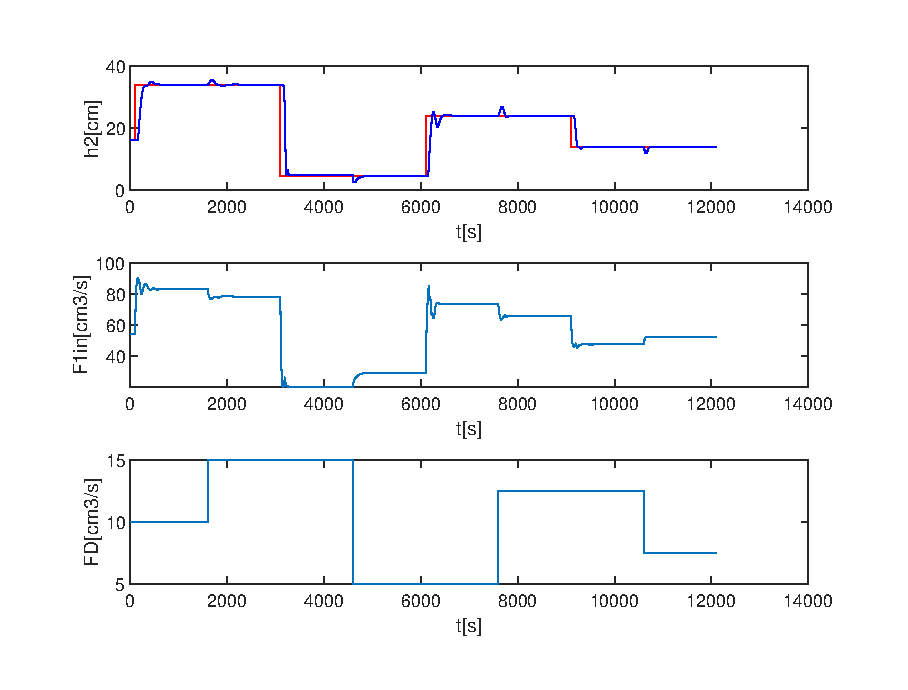
\includegraphics[width=0.9\linewidth]{plots/z3_fdmc_sl.eps}
		\caption{Przebieg regulacji dla numerycznego SL rozmytego}
		\label{rys:sl}
	\end{figure}
	
	
	Podczas sterowania regulatorem SL długości horyzontów, lambda oraz kształt funkcji przynależności przyjęte zostały takie same jak dla ostatniego przebiegu rozmytego regulatora DMC w zadaniu 2, czyli lambda równa 100, D równe 200, N równe 150, Nu równe 100, Dz równe 200 oraz funkcje przynależności tak jak na wykresie \ref{rys:dmcprzyn}.
	
	Przebieg regulacji umieszczony został an wykresie \ref{rys:sl}. Przebieg jest bardzo podobny do tego uzyskanego z rozmytego regulatora DMC, nie licząc okolic pierwszego skoku wartości zadanej wykresy praktycznie się nie różnią. Przy pierwszym skoku wartości zadanej algorytm SL działa jednakże nieco bardziej płynnie niż DMC. Przy regulacji DMC obiekt zwalnia przed dotarciem do wartości zadanej w formie pojedynczej oscylacji po czym dociera do niej praktycznie bez przeregulowania. Dla SL wykres jest płynniejszy, ale występuje wyraźne przekroczenie wartości zadanej. Błąd dla algorytmu SL wynosi jedynie 12.2571, więc jest zdecydowanie mniejszy niż błąd dla DMC. Oznacza to, że mimo wszystko wystąpiła poprawa regulacji.
	\chapter{Numeryczny rozmyty regulator NPL}
	Rozmyty regulator numeryczny NPL różni się od regulatora SL sposobem liczenia aktualnej odpowiedzi swobodnej. Wszystkie elementy odpowiedzi swobodnej liczy się rekurencyjnie za pomocą wzorów od \ref{eq:npl1} do \ref{eq:npl3}, przy czym przyszłe odpowiedzi modelu $y_{k+i}^M$ liczy się rekurencyjnie z modelu rozmytego obiektu, zakładając przyszłe przyrosty sterowania równe 0.	Dalsza praca regulatora postępuje tak jak dla algorytmu SL, włącznie z obliczaniem zmiany sterowania za pomocą funkcji optymalizacji.
	
	Podczas pracy regulatora wartości horyzontów, lambda oraz kształt funkcji przynależności przyjęte zostały takie jak dla regulatora SL.

	\begin{equation}
		y_{k+i|k}^0=y_{k+i}^M+dk;
		\label{eq:npl1}
	\end{equation}
	\begin{equation}
		d_k = y_k-\sum_{i=1}^{D-1}\tilde{s}_i*\Delta u_{k-i}-\tilde{s}_D*u_{k-D}
		%-\sum_{i=1}^{Dz-1}\tilde{s}_i^z*\Delta z_{k-i}-\tilde{s}_{Dz}^z*z_{k-Dz}
		\label{eq:npl2}
	\end{equation}
	\begin{equation}
		y_{k}^M = \sum_{i=1}^{D-1}\tilde{s}_i*\Delta u_{k-i}+\tilde{s}_D*u_{k-D}
		%+\sum_{i=1}^{Dz-1}\tilde{s}_i^z*\Delta z_{k-i}+\tilde{s}_{Dz}^z*z_{k-Dz}
		\label{eq:npl3}
	\end{equation}
	\chapter{Skrypty}
	\label{ch:skrypty}
	W celu uzyskania wykresów zamieszczonych w sprawozdaniu należy wywołać podane skrypty:
	\section{Zadanie 1}
	\begin{itemize}
		\item badanie modelu:\\
		$z1\_model$
		\item porównanie modelu nieliniowego i liniowego:\\
		$z1\_modellin$
		\item odpowiedź skokowa w punkcie pracy:\\
		$z1\_step(16, true)$
		\item przebiegi regulacji dla DMC:\\
		$z1\_dmc(400, 400, 400, 400, 100, true)$\\
		$z1\_dmc(400, 400, 400, 400, 1000, true)$\\
		$z1\_dmc(400, 400, 400, 400, 10000, true)$\\	
	\end{itemize}
	\section{Zadanie 2}
	\begin{itemize}
		\item obiekty rozmyte:\\
		$z2\_modelroz(2, true)$\\
		$z2\_modelroz(3, true)$\\
		$z2\_modelroz(4, true)$\\
		$z2\_modelroz(5, true)$\\
		\item dmc rozmyty, lambda 2000, oryginalne zbiory rozmyte:\\
		$z2\_dmcroz(400, 400, 400, 400, 2000,[],[], true)$
		\item dmc rozmyty, lambda 2000, nowe zbiory rozmyte:\\
		$z2\_dmcroz(400, 400, 400, 400, 2000,10,[8.5000   17.5000   24.5000   33.5000], true)$
		\item dmc rozmyty, lambda 100, nowe zbiory rozmyte:\\
		$z2\_dmcroz(400, 400, 400, 400, 100,10,[8.5000   17.5000   24.5000   33.5000], true)$
		\item dmc rozmyty, lambda 100, nowe zbiory rozmyte, skrócone horyzonty:\\
		$z2\_dmcroz(200, 150, 100, 200, 100,10,[8.5000   17.5000   24.5000   33.5000], true)$
	\end{itemize}
	\section{Zadanie 3}
	\begin{itemize}
		\item uruchomienie regulatora SL:\\
		$z3\_sl(200, 150, 100, 200, 100, true)$
	\end{itemize}
	
	\section{Zadanie 4}
	\begin{itemize}
		\item uruchomienie regulatora NPL:\\
		$z4\_npl(200, 150, 100, 200, 100, true)$
	\end{itemize}

\end{document}